\chapter{Formal Concept Analysis}
\label{chapter:formal-concept-analysis}

\FCA (henceforth initialised to FCA) is an approach to reasoning about \textit{concepts} and corresponding \textit{conceptual structures} in terms of lattice theory. At the foundation of FCA is a philosophical viewpoint, tracing back to Aristotle, which describes concepts as a unit consisting of two parts: the \textit{extension}, which refers to what one might refer to as instantiations of the concept, and the \textit{intension}, which refers to the meaning we ascribe to a concept by virtue of its properties \cite{ganter1999formal, WILLE1992493, DUQUENNE1999407}.

\section{Basic Notions in Formal Concept Analysis}
\label{section:basic-notions}

The starting point in FCA is almost always a structure called a \textit{formal context}, or simply a \textit{context}. A context describes a universe of discourse, as well as the underlying structural relationships that conceptual reasoning is based on.
%
\begin{definition}
\label{definition:formal-context} \index{formal context}
  A \textit{formal context} $\GMI$ is a triple comprised of a set $G$ of objects , a set $M$ of attributes, and a binary relation $I \subseteq G \times M$ referred to as an `incidence' relation. For an object-attribute pair $(g,m) \in I$ we might say that \say{Object $g$ \textit{has} the attribute $m$}.
\end{definition}

We regard the set of objects as being the extensional dimension of the context, while the set of attributes is intensional. However, this is largely convention; there is no strict requirement around what these sets are made up of, or that they be distinct. It is perfectly acceptable to have a context such as $(G,G,I)$ where the objects and attributes are the same set. \textcolor{red}{Perhaps add an intuition for what this context represents.}

It should be noted that, while the presence of an object--attribute pair $(g,m)$ in the incidence relation is interpreted as the object having the respective attribute, FCA is concerned with only \textit{positive} information, and so the absence of a pair in the relation is not usually interpreted to mean the object has the negation of the attribute. We will discuss the troubling matter of negative attributes in \Cref{section:contextual-attribute-logic}.

When the cardinalities of $G$ and $M$ are small, contexts may be represented as a cross-table such as in \Cref{context:formal-context-group-structures}. Each object is represented by a row in the table, each attribute by a column, and each element in the incidence relation is marked with an `$\times$' at the appropriate position \cite[pp. 17]{ganter1999formal}. Given a context that is presented in this form, it is quite trivial to identify all the attributes that a particular object satisfies: one need only scan across the respective row and note where the marks appear. The resulting set of attributes is called the \textit{object's intent}. The dual notion of an \textit{attribute extent} can be found by traversing down a column in the table.
\begin{example}
  \label{example:first-example-formal-context}
  Finite formal contexts of a reasonable size can be described entirely by a tabular representation. Each object corresponds to a row, and each attribute to a column in the table.

  \begin{figure}[H]
    \centering
    \small
    \begin{cxt}
    \label{cxt:grouplikes}
         \cxtName{\textbf{\texttt{Algebraic Structures}}}
      \att{\texttt{closure}} \att{\texttt{associativity}} \att{\texttt{identity}} \att{\texttt{divisibility}} \att{\texttt{commutativity}}
      \obj{x....}{\texttt{magma}}
      \obj{xx...}{\texttt{semigroup}}
      \obj{xxx..}{\texttt{monoid}}
      \obj{xxxx.}{\texttt{group}}
      \obj{xxxxx}{\texttt{abelian group}}
      \obj{x.xx.}{\texttt{loop}}
      \obj{x..x.}{\texttt{quasiagroup}}
      \obj{.xxx.}{\texttt{groupoid}}
      \obj{.xx..}{\texttt{category}}
      \obj{.x...}{\texttt{semicategory}}
    \end{cxt}
    \caption{A formal context showing necessary properties of group-like structures.}
    \label{context:formal-context-group-structures}
  \end{figure}
\end{example}

This approach to determining object extents and attribute intents becomes impractical when considering non-trivial contexts, or large sets of objects and attributes. The procedure can be formally described by the \textit{derivation operators}: \footnote{It is common to denote either derivation operator with a prime and use the surrounding context to resolve ambiguity, so $A^\uparrow$ and $B^\downarrow$ would become $A'$ and $B'$, respectively. We avoid this notation as later on it will become increasingly challenging to avoid ambiguity while maintaining pleasing notation. In cases where a derivation operator is applied to a singleton of objects $\{g\}$ (\textit{resp.} attributes $\{m\}$) we omit the parenthesis and write $g^\uparrow$ (\textit{resp.} $m^\downarrow$)}

\begin{definition}
     \label{definition:derivation-operators} \index{derivation operators}
  Given a context $\GMI$, the \textit{derivation operators} are two maps $(\cdot)^\uparrow : \pset{G} \to \pset{M}$ and $(\cdot)^\downarrow : \pset{M} \to \pset{G}$. Then, for any subsets $A \subseteq G$ and $B \subseteq M$,
  \begin{align*}
       A^\uparrow & \coloneqq \{m \in M \mid \forall g \in A, \; (g,m) \in I\} \\
       B^\downarrow & \coloneqq \{g \in G \mid \forall m \in B, \; (g,m) \in I\}
  \end{align*}
\end{definition}

The derivation operators offer a clear way to identify, for a given set $A \subseteq G$ of objects, the set $A^\uparrow$ of attributes which are common to each object in $A$. For example, the derivation of the set $\{\texttt{semigroup,monoid}\}$ of objects from \Cref{context:formal-context-group-structures} would be $\{\texttt{closure,associativity}\}$. In fact, we have already explored a more general perspective on the derivation operators in \Cref{section:closure-systems} through the notion of closure operators and Galois connections.

\begin{proposition}
\label{proposition:derivation-operators-galois}
Let $\GMI$ be a formal context and consider the subsets $X,X_1 \subseteq G$ of objects (\textit{resp.} $Y,Y_1 \subseteq M$ of attributes) then
\begin{align}
    & X \subseteq X_1 \Rightarrow X_1^\uparrow \subseteq X^\uparrow & \textit{(resp.)} & \qquad Y \subseteq Y_1 \Rightarrow Y_1^\downarrow \subseteq Y^\downarrow \label{equation:galois-1} \\
    & X \subseteq X^{\uparrow \downarrow} & \textit{(resp.)} & \qquad Y \subseteq Y^{\downarrow \uparrow} \label{equation:galois-2} \\
    & X^\uparrow = X^{\uparrow \downarrow \uparrow}  & \textit{(resp.)} & \qquad  Y^\downarrow = Y^{\downarrow \uparrow \downarrow} \label{equation:galois-3} \\
    & X \subseteq Y^\downarrow \Longleftrightarrow X^\uparrow \supseteq Y & \label{equation:galois-4}
\end{align}
\end{proposition}

If we consider the powerset lattices of $\pset{G}$ and $\pset{M}$ under the usual inclusion orders then the derivation operators constitute a Galois connection: \Cref{equation:galois-1,equation:galois-2,equation:galois-3} are just a  rephrasing of \Cref{equation:ord_galois-1,equation:ord-galois-2,equation:ord-galois-3}; and \Cref{equation:galois-4} rephrases \Cref{proposition:fundemental-galois}. Let us now consider some intution for why Galois connections appear when modelling concepts as the dual between extension and intension.

We have not yet formally defined concepts, but consider (under some common notion) the concept of a `human'. The size of this concept's extension---those things which may be considered instances of `human'---is quite large. Consider another concept, that of an `optometrist'. Presumably, the extension of the latter concept is contained within that of the former. While the intension---those properties we associate with an optometrist---would certainly be larger than, and more precisely a superset of, those associated with the concept of `human' (we hold the implicit view that only humans may be optemetrists). If we consider the shared properties of the extension of human, we should expect that it will at least contain `human'. Finally, once we have carefully amassed all the properties common to this extension, we should not expect any other extensional object we have not already considered to satisfy each of these properties, for it would then satisfy `human' and been included in our first consideration. \textcolor{red}{Perhaps this is a bit too basic, I can rephrase the intuition more technically and directly related to a context.}



From \Cref{proposition:derivation-operators-galois} we can describe two closure operators $(\cdot)^{\uparrow \downarrow}$ and $(\cdot)^{\downarrow \uparrow}$ on the powersets $\pset{G}$ and $\pset{M}$, respectively.



Of course, these two functions can be composed; and so, $A^{\uparrow \downarrow}$---which can rather cumbersomely be described as \say{The set of all objects which satisfy all the attributes satisfied by \texttt{semigroup} and \texttt{monoid}}---would yield the set $\{\texttt{semigroup, monoid, group, abelian group}\}$. In fact, this composition of derivation operators satisfies very specific properties.%

With the above relationship between sets of objets and attributes in mind, it is appropriate to introduce a \textit{formal concept}.

\begin{definition}
  \label{definition:formal-concept} \index{formal concept}
  A \textit{formal concept} of a formal context $\GMI$  is a pair $(A,B)$ of subsets $A \subseteq G$ and $B \subseteq M$ that satisfies $A^\uparrow = B$ and $B^\downarrow = A$. Then, we say that $A$ is the concept \textit{extent} and that $B$ is the \textit{intent}. We use $\BGMI$ to denote the set of all concepts of $\GMI$.
\end{definition}

\begin{example}
\label{example:formal-concept}
If we consider the \texttt{groupoid} object from \Cref{context:formal-context-group-structures}, we can derive the concept:

\[\big(\{\texttt{groupoid,group,abelian group}\}, \{\texttt{associativity,identity,closure}\} \big)\]

% The derivation of \texttt{groupoid} yields $\{\texttt{associativity,identity,closure}\}$, by \Cref{equation:galois-3} this set is closed under its Galois connection, and forms a concept intent.

% To begin, the object intent $\texttt{groupoid}^\uparrow$ is determined, which yields the set $\{\texttt{associativity,identity,closure}\}$. From \Cref{proposition:properties-about-derivation-operators} this set is closed, and represents a concept intent. The concept extent is determined by application of a derivation operator to the concept intent.
\end{example}

The set of all concepts has a natural ordering induced on it by the \textit{subconcept--superconcept} relation. If $(A_0,B_0)$ and $(A_1,B_1)$ are two concepts, then $(A_0,B_0)$ is a \textit{subconcept} of $(A_1, B_1)$ and $(A_1, B_1)$ is a superconcept of $(A_0,B_0)$ if and only if $A_0 \subseteq A_1$. Equivalently if $B_1 \subseteq B_0$. We denote set of all concepts ordered in this way by $\CLGMI$, and call this set the \textit{concept lattice} of $\GMI$.

Intuitively, one concept is a subconcept of another, if every instance of the first concept is also an instance of the second. From the Galois connection, this is equivalently, albeit less intuitively, explained by every attribute of the second concept being included in the first.

We can prescribe a rather intuitive ordering over concepts induced by the \textit{subconcept–superconcept} relation. \begin{figure}[H]
  \centering
  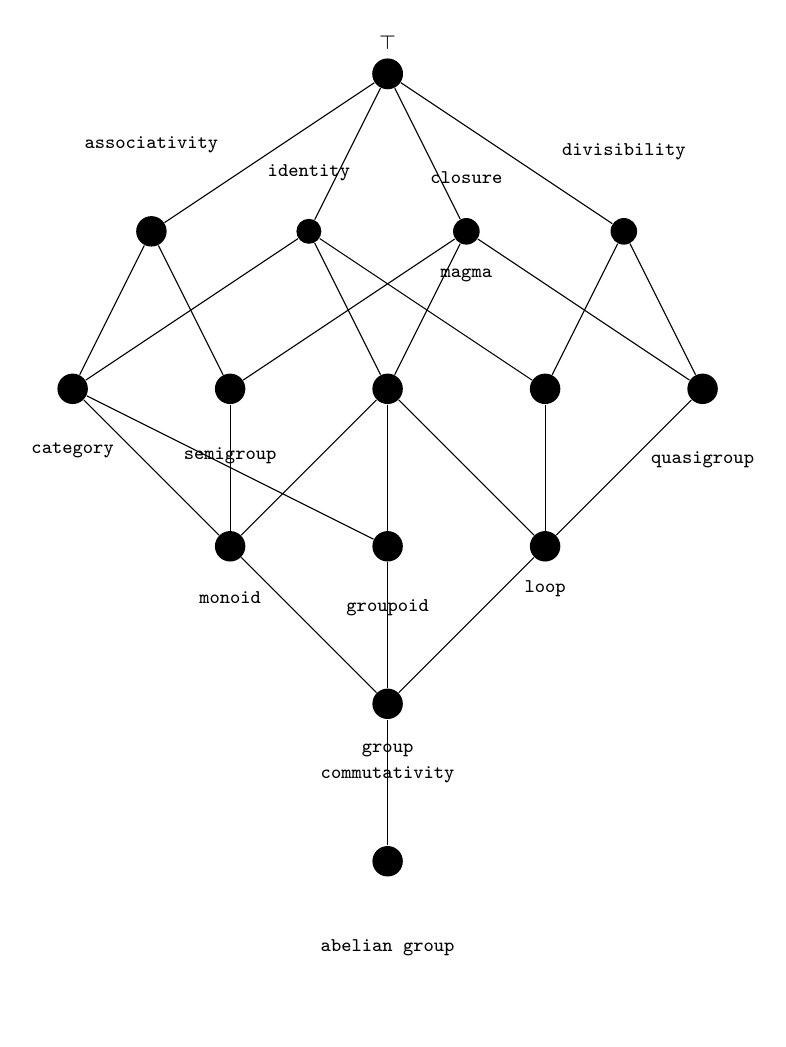
\begin{tikzpicture}[every node/.style={circle, fill=black, inner sep=1pt}]
    \node (a1) at (0,3) [label=above:{\scriptsize $\top$}] {w};
    % \node[draw=none, fill=none] at (0,3.5) {\tiny Top};

    \node (b1) at (-3,1) [label=above:{\scriptsize \texttt{associativity}}] {y};
    \draw (a1) -- (b1);

    \node (b2) at (-1,1) [label=above:{\scriptsize \texttt{identity}}] {z};
    \draw (a1) -- (b2);

    \node (b3) at (1,1) [label=above:{\scriptsize \texttt{closure}},label=below:{\scriptsize \texttt{magma}}] {x};
    \draw (a1) -- (b3);

    \node (b4) at (3,1) [label=above:{\scriptsize \texttt{divisibility}}] {x};
    \draw (a1) -- (b4);

    \node (c1) at (-4,-1) [label=below:{\scriptsize \texttt{category}}] {y};
    \draw (c1) -- (b1);
    \draw (c1) -- (b2);

    \node (c2) at (-2,-1) [label=below:{\scriptsize \texttt{semigroup}}] {y};
    \draw (c2) -- (b1);
    \draw (c2) -- (b3);

    \node (c3) at (0,-1) {y};
    \draw (c3) -- (b2);
    \draw (c3) -- (b3);

    \node (c4) at (2,-1) {y};
    \draw (c4) -- (b2);
    \draw (c4) -- (b4);

    \node (c5) at (4,-1) [label=below:{\scriptsize \texttt{quasigroup}}] {y};
    \draw (c5) -- (b3);
    \draw (c5) -- (b4);

    \node (d1) at (-2,-3) [label=below:{\scriptsize \texttt{monoid}}] {y};
    \draw (d1) -- (c1);
    \draw (d1) -- (c2);
    \draw (d1) -- (c3);

    \node (d2) at (0,-3) [label=below:{\scriptsize \texttt{groupoid}}] {y};
    \draw (d2) -- (c1);
    \draw (d2) -- (c3);

    \node (d3) at (2,-3) [label=below:{\scriptsize \texttt{loop}}] {y};
    \draw (d3) -- (c3);
    \draw (d3) -- (c4);
    \draw (d3) -- (c5);

    \node (e1) at (0,-5) [label=below:{\scriptsize \texttt{group}}] {y};
    \draw (e1) -- (d1);
    \draw (e1) -- (d2);
    \draw (e1) -- (d3);

    \node (f1) at (0,-7)[label=above:{\scriptsize \texttt{commutativity}},label=below:{\scriptsize \texttt{abelian group}}] {y};
    \draw (f1) -- (e1);
  \end{tikzpicture}
  \caption{The concept lattice associated with the formal context in \Cref{context:formal-context-group-structures}}
\end{figure}

\subsection{Attribute Implications}
\label{subsection:attribute-implications}

In FCA, attribute implications represent dependencies that exist between attributes in a context. If $M$ is a non-empty set of attributes with $A, B \subseteq M$, then we denote an attribute implication over $M$ as $A \rightarrow B$.

\begin{definition}
     \label{definition:attribute-implication}
     Let $M$ be a non-empty set of attributes, then an \emph{attribute implication} over $M$ is a
\end{definition}


If we examine the context in \Cref{context:voting-records-small} it is apparent that every representative who voted in favour of the proposed crime bill also voted in favour of the immigration bill; we write this dependency as $\texttt{crime} \rightarrow \texttt{immigration}$.



\begin{figure}[H]
\centering
    \begin{cxt}
         \cxtName{\textbf{\texttt{Congressional Voting Records}}}
         \atr{\texttt{mx-missile}}
         \atr{\texttt{crime}}
         \atr{\texttt{immigration}}
         \atr{\texttt{satellite ban}}
         \atr{\texttt{education}}
         \atr{\texttt{republican}}
         \atr{\texttt{democrat}}
         \obj{.xx.xx.}{\texttt{Representative 1}}
         \obj{......x}{\texttt{Representative 4}}
         \obj{.x..xx.}{\texttt{Representative 9}}
         \obj{..x.x.x}{\texttt{Representative 17}}
    \end{cxt}
    \caption{A context describing a portion of congressional voting records for 1984}
    \label{context:voting-records-small}
\end{figure}

\clearpage

\section{Contextual Attribute Logic}
\label{section:contextual-attribute-logic}

The attribute logic that usually underlies any discussion on FCA is analagous to Horn logic. Attribute implications are quite easily shown to be analagous to propositional Horn clauses: If we consider the (attribute) implication $A \rightarrow B$, with $A, B \subseteq M$ it can be phrased, with respect to holding in a context $\GMI$, as \say{all objects which satisfy every attribute in $A$ also satisfy every attribute in $B$}.

The underlying logic we have just described for FCA can quite easily be shown to be analagous to propositional Horn logic. Horn rules are syntactically similar to material implications, and share the same `$\rightarrow$' operator. However, none of the premise nor conclusion of a Horn rule may be negative, or contain disjunction. They are not able to express what is \textit{not} a consequence of a premise.
